\subsection{Asesor}

  \paragraph{}Se procede a crear el usuario asesor, en este caso José Manuel,
  cuyo DNI es 99887766Z y su correo electrónico es \textit{jm\_bio@uco.es}. Para
  ello, se realizará la creación de un asesor, tal y como se describió en el
  capítulo \ref{addAsesor}, \textit{Añadir asesor}.

  \paragraph{}Una vez que aparezca el formulario de creación, se debe introducir
  el nombre del asesor, su DNI y correo electrónico en el formulario, con lo que
  la pantalla quedaría tal y como refleja la figura \ref{ejemploAddAsesor}.

  \begin{figure}[!ht]
    \begin{center}
      \fbox{
      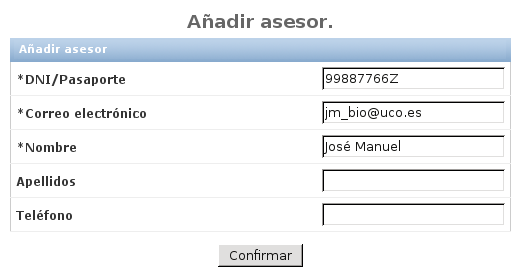
\includegraphics[scale=0.55]{5.Ejemplos_Practicos/5.3.IntroduccionDatos/5.3.6.Asesor/add_asesor.png}
      }
      \caption{Creación de \textit{Asesor} de ejemplo.}
      \label{ejemploAddAsesor}
    \end{center}
  \end{figure}

  \paragraph{}Una vez rellenado el formulario, se pulsará el botón
  \textit{Confirmar}, el cual se puede ver en la figura
  \ref{capturaBotonConfirmar}. Si el formulario rellenado es válido, y no tiene
  errores, se creará el nuevo elemento en el sistema. En caso de contener
  información no válida, un mensaje de error aparecerá indicando los campos
  del formulario que no han pasado la validación, los cuales habrá que modificar
  para introducir correctamente el elemento en el sistema.
